\documentclass[conference]{IEEEtran}
\IEEEoverridecommandlockouts

\usepackage{cite}
\usepackage{amsmath,amssymb,amsfonts}
\usepackage{algorithm}
\usepackage{algpseudocode}
\usepackage{graphicx}
\usepackage{textcomp}
\usepackage{xcolor}
\usepackage{booktabs}
\usepackage{multirow}
\usepackage{array}
\usepackage{tikz}
\usetikzlibrary{arrows.meta,positioning,fit,backgrounds,calc,shapes.geometric}
\usepackage{pgfplots}
\pgfplotsset{compat=1.18}
\usepackage[hidelinks]{hyperref}
\hypersetup{
  pdftitle={Searching Code Repositories with Natural-Language Queries},
  pdfauthor={Anuran Basu, Bornik Roychowdry, Samarth Patel},
  pdfcreator={LaTeX}
}

% generated by report/make_numbers.py -- do not edit
\newcommand{\NQueries}{42}
\newcommand{\DenseAccOne}{0.714}
\newcommand{\DenseMRR}{0.813}
\newcommand{\DenseRFive}{0.940}
\newcommand{\LexAccOne}{0.286}
\newcommand{\LexMRR}{0.474}
\newcommand{\LexRFive}{0.726}
\newcommand{\QWords}{12.6}
\newcommand{\QWordsMin}{8}
\newcommand{\QWordsMax}{19}
\newcommand{\NTargets}{44}
\newcommand{\FalseEdges}{28}
\newcommand{\FalseEdgePct}{8.2}
\newcommand{\HybFiveP}[1]{\csname hybp#1\endcsname}
\newcommand{\HybFiveR}[1]{\csname hybr#1\endcsname}
\newcommand{\HybFiveF}[1]{\csname hybf#1\endcsname}
\expandafter\def\csname hybp3\endcsname{0.302}
\expandafter\def\csname hybr3\endcsname{0.869}
\expandafter\def\csname hybf3\endcsname{0.445}
\expandafter\def\csname hybp5\endcsname{0.195}
\expandafter\def\csname hybr5\endcsname{0.940}
\expandafter\def\csname hybf5\endcsname{0.322}
\expandafter\def\csname hybp10\endcsname{0.100}
\expandafter\def\csname hybr10\endcsname{0.964}
\expandafter\def\csname hybf10\endcsname{0.181}
\newcommand{\MainRows}{BM25 (lexical) & 0.286 & 0.214 & 0.631 & 0.319 & 0.148 & 0.726 & 0.245 & 0.869 & 0.163 & 0.474 & 0.565 \\
Dense (CodeRankEmbed) & \textbf{0.714} & 0.302 & 0.869 & 0.445 & \textbf{0.195} & \textbf{0.940} & \textbf{0.322} & \textbf{0.964} & \textbf{0.181} & 0.813 & 0.847 \\
Hybrid RRF ($\lambda_{\text{lex}}=1$) & 0.595 & \textbf{0.310} & \textbf{0.893} & \textbf{0.457} & 0.186 & 0.893 & 0.306 & 0.940 & 0.176 & 0.741 & 0.789 \\
Hybrid RRF ($\lambda_{\text{lex}}=0.05$) & \textbf{0.714} & 0.302 & 0.869 & 0.445 & \textbf{0.195} & \textbf{0.940} & \textbf{0.322} & \textbf{0.964} & \textbf{0.181} & \textbf{0.814} & \textbf{0.848} \\}
\newcommand{\SigHybP}{0.054}
\newcommand{\AblRows}{Full system & 1307 & 0.714 & 0.940 & 0.813 & 0.847 \\
$-$ contextual header & 1307 & 0.786 & 0.881 & 0.842 & 0.868 \\
Fixed 60-line windows & 781 & 0.524 & 0.857 & 0.651 & 0.705 \\
\midrule
BM25, syntax chunks & 1307 & 0.286 & 0.726 & 0.474 & 0.565 \\
BM25, 60-line windows & 781 & 0.262 & 0.667 & 0.442 & 0.533 \\}
\newcommand{\WinDRFive}{8.3}
\newcommand{\AblText}{\textbf{Syntax-aware chunking.} Replacing definition-level chunks by fixed 60-line windows (with 10 lines of overlap) reduces dense Acc@1 from 0.714 to 0.524, Recall@5 from 0.940 to 0.857 and MRR@10 from 0.813 to 0.651 ($p = 0.017$, Table~\ref{tab:sig}). BM25 also degrades (MRR@10 0.474 $\rightarrow$ 0.442). The drop occurs although the evaluation is lenient towards windows: a window counts as relevant whenever it overlaps the target definition, even if most of it is unrelated code. Windows mix several definitions into one vector, and their headers carry no symbol name. \textbf{Contextual header.} Removing the \texttt{File:}/\texttt{Symbol:} header gives a mixed result: Acc@1 rises from 0.714 to 0.786 and MRR@10 from 0.813 to 0.842, but Recall@5 falls from 0.940 to 0.881. The difference in reciprocal rank is not significant ($p = 0.479$; 5 queries improve and 4 worsen). The changed queries show two opposing effects. With the header, short definitions whose symbol names contain query words rank higher; for the template-loader query, \texttt{Blueprint.app\_template\_global} outranks the correct \texttt{DispatchingJinjaLoader} (rank 9 vs.\ rank 1 without header). Without the header, tests and documentation describing the same behaviour rank above the implementation; \texttt{test\_blueprint\_prefix\_slash} displaces \texttt{BlueprintSetupState.add\_url\_rule} (rank 6 vs.\ rank 1 with header). The header is therefore not a reliable improvement for this model and benchmark.}
\newcommand{\CastCompare}{Syntax-aware vs.\ 60-line windows: +8.3 Recall@5 points (dense retrieval, Flask)}
\newcommand{\CastDiscussion}{Zhang \emph{et al.} report that AST-based chunking improves Recall@5 by 4.3 points over fixed-size chunking on RepoEval. Our ablation points in the same direction with a larger effect, +8.3 Recall@5 points and +0.162 MRR@10. The settings differ (RepoEval targets code completion with code queries, whereas our queries are natural language and our windows are line-based rather than size-balanced), so the magnitudes are not directly comparable, but both studies indicate that chunk boundaries aligned with the syntax tree matter for code retrieval.}
\newcommand{\AblConclusion}{Syntax-aware chunking is essential: fixed windows lower Recall@5 by 8.3 points, in line with prior work on AST chunking, whereas the contextual header has no significant effect.}
\newcommand{\HoSha}{14459c77d379}
\newcommand{\HoQueries}{30}
\newcommand{\GBeta}{0.5}
\newcommand{\GTop}{5}
\newcommand{\GTestW}{0.5}
\newcommand{\HoRows}{BM25 & 0.286 & 0.726 & 0.474 & 0.565 & 0.433 & 0.700 & 0.551 & 0.611 \\
Dense & 0.714 & 0.940 & 0.813 & 0.847 & 0.767 & 0.933 & 0.823 & 0.857 \\
Hybrid ($\lambda_{\text{lex}}{=}1$) & 0.595 & 0.893 & 0.741 & 0.789 & 0.700 & 0.933 & 0.769 & 0.809 \\
\midrule
BM25 + graph & -- & -- & -- & -- & 0.500 & 0.733 & 0.600 & 0.656 \\
Dense + graph & 0.690 & 0.940 & 0.801 & 0.839 & 0.833 & 0.967 & 0.879 & 0.901 \\
Hybrid + graph & 0.571 & 0.917 & 0.730 & 0.781 & 0.700 & 0.933 & 0.769 & 0.809 \\}
\newcommand{\HoDenseMRR}{0.823}
\newcommand{\HoHybMRR}{0.769}
\newcommand{\HoLexMRR}{0.551}
\newcommand{\HoGDenseMRR}{0.879}
\newcommand{\HoDenseAcc}{0.767}
\newcommand{\HoGDenseAcc}{0.833}
\newcommand{\DevGDenseMRR}{0.801}
\newcommand{\SweepFiveFull}{(0.5,0.7951) (1.0,0.7385) (2.0,0.7075) (4.0,0.6204)}
\newcommand{\SweepFiveHalf}{(0.5,0.8010) (1.0,0.7447) (2.0,0.7138) (4.0,0.6259)}
\newcommand{\SweepTenFull}{(0.5,0.7384) (1.0,0.6336) (2.0,0.5884) (4.0,0.4673)}
\newcommand{\SweepTenHalf}{(0.5,0.7435) (1.0,0.6398) (2.0,0.5937) (4.0,0.4718)}
\newcommand{\SweepBase}{0.8130}
\newcommand{\GDevDelta}{-0.012}
\newcommand{\GDevP}{0.489}
\newcommand{\GDevWL}{3/2}
\newcommand{\GHoDelta}{+0.056}
\newcommand{\GHoP}{0.128}
\newcommand{\GHoWL}{4/0}
\newcommand{\GPoolDelta}{+0.017}
\newcommand{\GPoolP}{0.325}
\newcommand{\GPoolWL}{7/2}
\newcommand{\HoDenseVsHybP}{0.416}
\newcommand{\SigRows}{Dense vs.\ BM25 & +0.339 & $<$0.001 & 25 / 4 \\
Dense vs.\ hybrid ($\lambda{=}1$) & +0.072 & 0.054 & 9 / 4 \\
Hybrid ($\lambda{=}0.05$) vs.\ dense & +0.001 & 1.000 & 1 / 0 \\
Syntax chunks vs.\ windows (dense) & +0.162 & 0.017 & 15 / 5 \\
No header vs.\ header (dense) & +0.029 & 0.479 & 5 / 4 \\
Graph rerank, dense (dev) & -0.012 & 0.489 & 3 / 2 \\
Graph rerank, dense (held-out) & +0.056 & 0.128 & 4 / 0 \\
Graph rerank, dense (pooled, $n{=}72$) & +0.017 & 0.325 & 7 / 2 \\}
\newcommand{\QueryLatency}{Loading the encoder takes 12.1\,s once per process; after that a query takes a median of 177\,ms in dense mode, 180\,ms in hybrid mode and 3.8\,ms for BM25 alone (42 queries); the additional cost of dense retrieval covers query encoding and the exhaustive scan.}


\newcommand{\sys}{\textsc{CodeRet}}

\begin{document}

\title{Searching Code Repositories with\\ Natural-Language Queries}

\author{\IEEEauthorblockN{Anuran Basu, Bornik Roychowdry and Samarth Patel}}

\maketitle

% ---------------------------------------------------------------------------
\begin{abstract}
Developers spend a large share of their time locating the code that implements
a behaviour they can describe only in natural language. We present \sys{}, an
offline repository-level code retrieval system designed for reproducible
experimentation on CPU-only hardware. \sys{} segments source files into
definition-level chunks with tree-sitter, extracts a dependency graph of
definitions, call references and resolved imports, and combines an exact,
memory-bounded dense scan over CodeRankEmbed embeddings with BM25, fused by
weighted reciprocal rank fusion. Embeddings are cached under a content hash, so
re-indexing reuses every unchanged vector. We also propose \emph{test-aware graph
reranking}, which uses the extracted call graph to promote the implementation
code exercised by test functions that rank highly. We evaluate on \NQueries{}
development and \HoQueries{} held-out natural-language queries over the Flask web
framework. Dense retrieval reaches a top-1 accuracy of \DenseAccOne{} and an
MRR@10 of \DenseMRR{}, against \LexAccOne{} and \LexMRR{} for BM25, and the
ranking dense $>$ hybrid $>$ BM25 replicates on the held-out set. Equal-weight
hybrid fusion lowers top-1 accuracy relative to dense retrieval alone, and
replacing syntax-aware chunks with fixed line windows lowers Recall@5 by
\WinDRFive{} points ($p = 0.017$). Test-aware reranking, tuned on the
development set only, raises held-out MRR@10 from \HoDenseMRR{} to
\HoGDenseMRR{} (4 queries improved, none worsened) but slightly lowers
development MRR@10; the effect is not statistically significant ($p = \GPoolP{}$
pooled). An audit of import resolution shows that a package-aware rule removes
all \FalseEdges{} false-positive dependency edges produced by naive path matching.
\end{abstract}

\begin{IEEEkeywords}
code search, information retrieval, dense retrieval, BM25, rank fusion,
abstract syntax tree, dependency analysis, reproducibility
\end{IEEEkeywords}

% ---------------------------------------------------------------------------
\section{Introduction}

\subsection{Background}
Code search is one of the most frequent activities in software development:
before changing a system, a developer must find where a behaviour is
implemented, which functions call it and which modules it depends on. Keyword
tools such as \texttt{grep} work only when the developer already knows the
identifiers involved. Natural-language queries such as ``where is the session
cookie signed'' require a retriever that maps descriptions to code.

Learned code representations have made this possible. Early neural approaches
embedded code and descriptions in a joint space~\cite{gu2018deep}, and the
CodeSearchNet challenge~\cite{husain2019codesearchnet} established a large
benchmark for the task. Pre-trained models such as CodeBERT~\cite{feng2020codebert}
and UniXcoder~\cite{guo2022unixcoder} improved semantic matching further, and
contrastively trained retrievers such as CodeRankEmbed~\cite{suresh2025cornstack}
now lead benchmarks such as CoIR~\cite{li2025coir}.

\subsection{Importance and Motivation}
Retrieval is also the first stage of retrieval-augmented generation
(RAG)~\cite{lewis2020rag}, where the quality of the retrieved context bounds the
quality of any downstream answer, and of repository-level tasks such as issue
resolution~\cite{jimenez2024swebench} and code completion~\cite{zhang2023repocoder}.
Yet three practical gaps remain between benchmark models and usable research
tools:
\begin{enumerate}
  \item \emph{Hardware.} Most pipelines assume a GPU and approximate
        nearest-neighbour (ANN) indexes, which trade recall for speed and make
        results depend on index parameters.
  \item \emph{Granularity.} Benchmarks evaluate on pre-extracted functions,
        whereas real repositories must first be chunked. Fixed-size chunking
        splits functions across chunks~\cite{zhang2025cast}.
  \item \emph{Structure.} A ranked list of snippets does not tell a developer
        who calls a function or which file an import refers to.
\end{enumerate}
Our motivation is a tool that a researcher can run on an ordinary laptop,
that gives exact and reproducible rankings, and that combines semantic search
with the dependency structure of the repository.

\subsection{Contributions}
\begin{itemize}
  \item \textbf{System.} \sys{}, an open, CPU-only retrieval system with
        tree-sitter chunking for 12 languages, dependency extraction, exact
        streaming dense search, BM25, weighted reciprocal rank fusion and a
        content-addressed embedding cache with incremental, resumable indexing.
  \item \textbf{Test-aware graph reranking.} A lightweight reranker that uses the
        extracted call graph to redirect relevance from test functions to the
        implementation code they exercise, requiring no additional model.
  \item \textbf{Benchmark and protocol.} \NQueries{} development and \HoQueries{}
        held-out labelled queries over a pinned revision of Flask. Labels are
        resolved to definition spans, so they remain valid across chunking
        strategies, and all tuning is restricted to the development set.
  \item \textbf{Empirical findings.} A controlled comparison of dense, lexical
        and hybrid retrieval with a fusion-weight sweep, ablations of chunking
        and contextual headers, paired significance tests, replication on held-out
        queries, and a comparison with published results.
  \item \textbf{Dependency audit.} A measurement showing that path-suffix import
        matching produces \FalseEdgePct{}\% false-positive edges, and a
        package-aware rule, following Python's import semantics, that removes them.
\end{itemize}

% ---------------------------------------------------------------------------
\section{Literature Review}

\textbf{Neural code search.} Gu \emph{et al.}~\cite{gu2018deep} introduced
DeepCS, which embeds code snippets and natural-language descriptions into a
shared vector space with recurrent encoders and ranks code by cosine
similarity. Husain \emph{et al.}~\cite{husain2019codesearchnet} released
CodeSearchNet, about two million function--docstring pairs in six languages
with expert-annotated queries, which became the standard benchmark and
popularised MRR as its metric.

\textbf{Pre-trained code models.} CodeBERT~\cite{feng2020codebert} pre-trained
a bimodal Transformer on code and text with masked-language and
replaced-token-detection objectives. UniXcoder~\cite{guo2022unixcoder} unified
encoder and decoder modes and added contrastive learning over abstract syntax
tree (AST) and comment views, which substantially improved zero-shot code
search.

\textbf{Dense retrieval and contrastive data.} Dense passage
retrieval~\cite{karpukhin2020dpr} showed that a dual encoder trained with
in-batch negatives can outperform BM25 for open-domain question answering.
For code, CoRNStack~\cite{suresh2025cornstack} curated 21 million
consistency-filtered text--code pairs with mined hard negatives and trained
CodeRankEmbed, a 137M-parameter retriever reporting 77.9 MRR on CodeSearchNet
and 60.1 nDCG@10 on CoIR. CoIR~\cite{li2025coir} aggregates ten code retrieval
datasets across eight tasks and uses nDCG@10 as its primary metric.

\textbf{Lexical retrieval and fusion.} BM25~\cite{robertson2009bm25} remains a
strong baseline whenever queries share vocabulary with documents. Reciprocal
rank fusion (RRF)~\cite{cormack2009rrf} combines rankings using only their
ranks and was reported to outperform both Condorcet fusion and the individual
input systems. Cross-encoder rerankers~\cite{nogueira2019passage} rescore a
candidate pool with full query--document attention.

\textbf{Repository-level retrieval.} RAG~\cite{lewis2020rag} conditions
generation on retrieved passages. RepoCoder~\cite{zhang2023repocoder} applies
iterative retrieval to repository-level code completion, and
SWE-bench~\cite{jimenez2024swebench} evaluates issue resolution on real GitHub
repositories, where localising the relevant files is a key sub-problem. cAST~\cite{zhang2025cast}
showed that splitting code along AST boundaries instead of fixed line counts
raises Recall@5 by 4.3 points on RepoEval.

\textbf{Graph-based retrieval and test-to-code links.} Several systems
exploit code structure during retrieval. RepoHyper~\cite{phan2024repohyper}
builds a repository-level semantic graph and expands and reranks retrieved
snippets by link prediction, and GraphCoder~\cite{liu2024graphcoder} retrieves
context by matching code context graphs of control and data dependences; both
target code completion. In software engineering, TCTracer~\cite{white2022tctracer}
establishes traceability links between tests and the functions they test using
static and dynamic call information, and applies them to traceability and
maintenance tasks rather than to search.

\textbf{Positioning of this work.} The individual components of \sys{} are
established: syntax-aware chunking~\cite{zhang2025cast}, hybrid retrieval with
rank fusion~\cite{cormack2009rrf} and graph-based context
retrieval~\cite{phan2024repohyper,liu2024graphcoder}, and open-source developer
tools also offer local semantic code search. Our contributions are (i)~a
reproducible, exact, CPU-only system that integrates these components with a
dependency graph; (ii)~an evaluation protocol whose labels are resolved through
extracted definitions, which makes chunking strategies directly comparable on the
same queries; (iii)~test-aware graph reranking, which applies test-to-code call
links to natural-language code search, a combination we did not find in the
literature we reviewed; and (iv)~a set of controlled measurements, including
negative and inconclusive results, on a development set and a held-out set.

% ---------------------------------------------------------------------------
\section{Objective}
The objectives of this work are:
\begin{enumerate}
  \item To build a repository-level code retrieval system that runs entirely on
        a CPU without approximate indexing and without reduced-precision
        inference.
  \item To segment code into semantically coherent units and to extract a
        correct dependency graph of definitions, calls and imports.
  \item To support incremental, resumable indexing in which no unchanged code
        is ever re-embedded.
  \item To measure, on a labelled benchmark, the accuracy of dense, lexical and
        hybrid retrieval, and the effect of chunking and contextual headers.
  \item To test whether the extracted call graph can improve ranking by
        redirecting relevance from tests to the code they exercise, with
        held-out evaluation.
  \item To make every experiment reproducible from a configuration fingerprint,
        a pinned model revision and a pinned corpus revision.
\end{enumerate}

% ---------------------------------------------------------------------------
\section{Proposed Model}

Fig.~\ref{fig:arch} shows the architecture. The \emph{indexing path} (top)
turns a repository into chunks, a dependency graph and cached embeddings. The
\emph{query path} (bottom) retrieves with two independent rankers and fuses
their results.

\begin{figure*}[t]
\centering
\resizebox{\textwidth}{!}{%
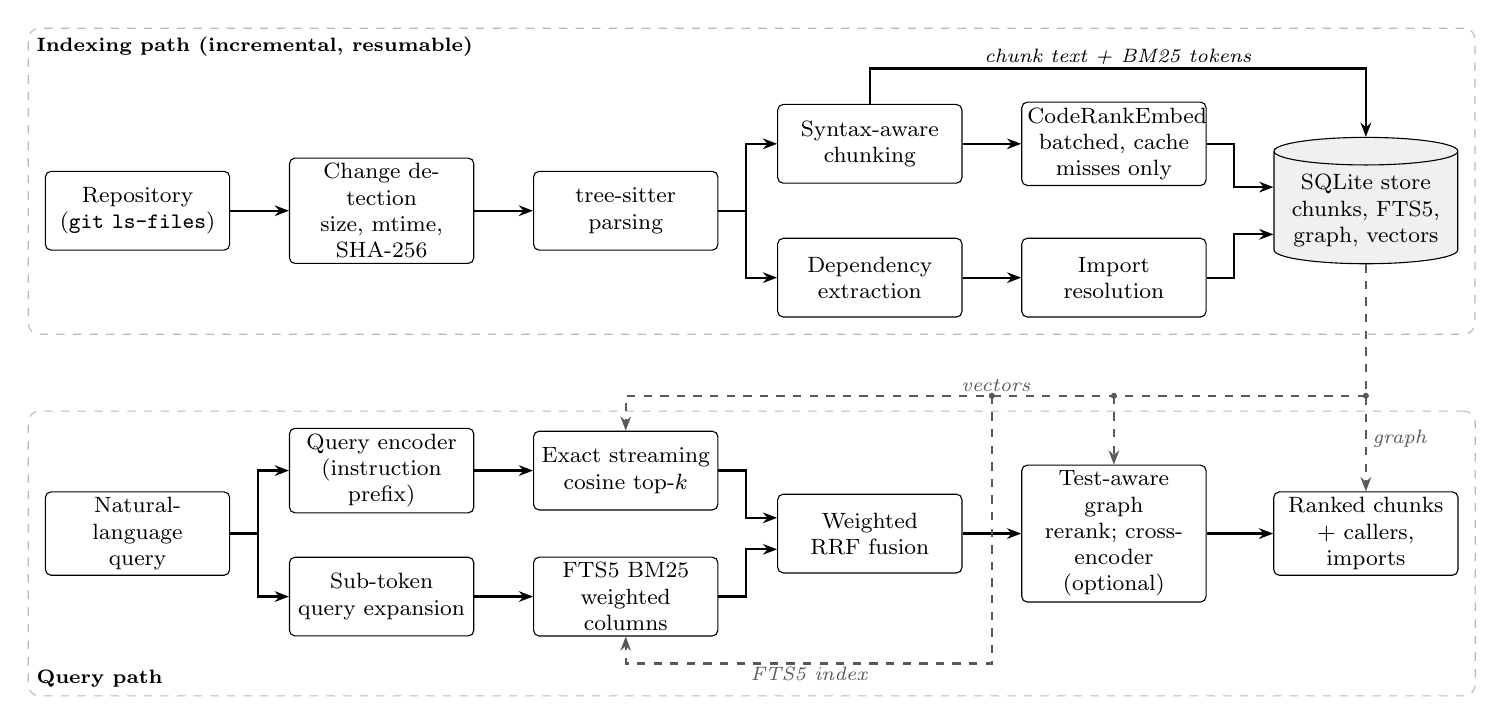
\begin{tikzpicture}[
  font=\footnotesize,
  box/.style={draw, rounded corners=2pt, align=center, text width=22mm,
              minimum height=10mm, fill=white, inner sep=2pt},
  store/.style={draw, cylinder, shape border rotate=90, aspect=0.15, align=center,
                text width=21mm, minimum height=16mm, fill=gray!12},
  arr/.style={-{Stealth[length=1.8mm]}, thick},
  db/.style={-{Stealth[length=1.8mm]}, thick, dashed, gray!70!black},
  lab/.style={font=\scriptsize\itshape, fill=white, inner sep=1pt},
  lane/.style={draw=gray!55, dashed, rounded corners=4pt, inner sep=6pt}
]
% ---------------- indexing path (y = 0) ----------------
\node[box] (repo)  at (0,0)     {Repository\\(\texttt{git ls-files})};
\node[box] (chg)   at (3.1,0)   {Change detection\\size, mtime, SHA-256};
\node[box] (ts)    at (6.2,0)   {tree-sitter\\parsing};
\node[box] (chunk) at (9.3,0.85)  {Syntax-aware\\chunking};
\node[box] (deps)  at (9.3,-0.85) {Dependency\\extraction};
\node[box] (emb)   at (12.4,0.85) {CodeRankEmbed\\batched, cache\\misses only};
\node[box] (res)   at (12.4,-0.85){Import\\resolution};
\node[store] (db)  at (15.6,0)  {SQLite store\\chunks, FTS5,\\graph, vectors};

\draw[arr] (repo) -- (chg);
\draw[arr] (chg) -- (ts);
\draw[arr] (ts.east) -- ++(0.35,0) |- (chunk.west);
\draw[arr] (ts.east) -- ++(0.35,0) |- (deps.west);
\draw[arr] (chunk) -- (emb);
\draw[arr] (deps) -- (res);
\draw[arr] (emb.east) -- ++(0.35,0) |- ([yshift=3mm]db.west);
\draw[arr] (res.east) -- ++(0.35,0) |- ([yshift=-3mm]db.west);
\draw[arr] (chunk.north) -- ++(0,0.45) -| node[lab, pos=0.25, above]{chunk text + BM25 tokens} (db.north);

% ---------------- query path (y = -4) ----------------
\node[box] (q)     at (0,-4.1)    {Natural-language\\query};
\node[box] (qe)    at (3.1,-3.3)  {Query encoder\\(instruction prefix)};
\node[box] (sub)   at (3.1,-4.9)  {Sub-token\\query expansion};
\node[box] (dense) at (6.2,-3.3)  {Exact streaming\\cosine top-$k$};
\node[box] (lex)   at (6.2,-4.9)  {FTS5 BM25\\weighted columns};
\node[box] (rrf)   at (9.3,-4.1)  {Weighted\\RRF fusion};
\node[box] (rr)    at (12.4,-4.1) {Test-aware graph\\rerank; cross-\\encoder (optional)};
\node[box] (out)   at (15.6,-4.1) {Ranked chunks\\+ callers, imports};

\draw[arr] (q.east) -- ++(0.35,0) |- (qe.west);
\draw[arr] (q.east) -- ++(0.35,0) |- (sub.west);
\draw[arr] (qe) -- (dense);
\draw[arr] (sub) -- (lex);
\draw[arr] (dense.east) -- ++(0.35,0) |- ([yshift=2mm]rrf.west);
\draw[arr] (lex.east) -- ++(0.35,0) |- ([yshift=-2mm]rrf.west);
\draw[arr] (rrf) -- (rr);
\draw[arr] (rr) -- (out);

% ---------------- reads from the store ----------------
\coordinate (j) at (15.6,-2.35);
\draw[db] (db.south) -- (j) -- (out.north) node[lab, pos=0.45, right=1pt]{graph};
\draw[db] (j) -| node[lab, pos=0.25, above]{vectors} (dense.north);
\draw[db] (10.85,-2.35) -- (10.85,-5.75) -| node[lab, pos=0.25, below]{FTS5 index} (lex.south);
\fill[gray!70!black] (10.85,-2.35) circle (1.1pt);
\draw[db] (12.4,-2.35) -- (rr.north);
\fill[gray!70!black] (12.4,-2.35) circle (1.1pt);
\fill[gray!70!black] (j) circle (1.1pt);

\coordinate (toplane) at ($(chunk.north)+(0,0.75)$);
\begin{scope}[on background layer]
\node[lane, fit=(repo)(chunk)(deps)(db)(emb)(toplane)] (L1) {};
\node[anchor=north west, font=\scriptsize\bfseries, inner sep=3pt] at (L1.north west) {Indexing path (incremental, resumable)};
\coordinate (botlane) at (6.2,-5.95);
\node[lane, fit=(q)(qe)(sub)(out)(rr)(botlane)] (L2) {};
\node[anchor=south west, font=\scriptsize\bfseries, inner sep=3pt] at (L2.south west) {Query path};
\end{scope}
\end{tikzpicture}}
\caption{Architecture of \sys{}. Solid arrows show data flow; dashed arrows show
reads from and writes to the single SQLite store. Only changed files are
parsed, and only chunks whose content hash is absent from the cache are
embedded.}
\label{fig:arch}
\end{figure*}

The process has six stages:
\begin{enumerate}
  \item \textbf{Discovery.} Tracked and untracked, non-ignored files are listed
        with \texttt{git ls-files}; binary and oversized files are skipped.
  \item \textbf{Change detection.} A file is re-parsed only if its size or
        modification time changed \emph{and} its SHA-256 differs from the stored
        digest. Deleted files are removed. A fingerprint of the chunking settings
        forces a full re-parse when those settings change.
  \item \textbf{Parsing and chunking.} Each file is parsed once with
        tree-sitter and split into definition-level chunks (Section~\ref{sec:chunking}).
  \item \textbf{Dependency extraction.} The same syntax tree yields definitions
        with qualified names, call references and import statements, which are
        resolved to files (Section~\ref{sec:deps}).
  \item \textbf{Embedding.} Chunks lacking a vector for the active model are
        embedded in batches, and each batch is committed immediately, so an
        interrupted run resumes where it stopped.
  \item \textbf{Retrieval.} A query is answered by exact dense search and BM25,
        fused by weighted RRF (Section~\ref{sec:retrieval}), and optionally
        reranked using the call graph (Section~\ref{sec:graphrr}) or a
        cross-encoder.
\end{enumerate}

% ---------------------------------------------------------------------------
\section{Methodology}

\subsection{Syntax-Aware Chunking}\label{sec:chunking}
Let $L$ be the character budget of a chunk ($L = 3000$). Algorithm~\ref{alg:chunk}
recursively assigns each outermost definition (function, class, method,
including decorators and export wrappers) to its own chunk. Oversized
definitions that contain nested definitions, typically large classes, are split
into one chunk per nested definition plus a \emph{header} chunk holding the
remaining lines (signature, docstring, attributes). Oversized definitions without
nested definitions are split into overlapping windows of $w = 60$ lines with
overlap $o = 10$. Lines outside any definition (imports, globals, scripts)
form contiguous \emph{module} chunks. Each chunk records its qualified symbol
(e.g.\ \texttt{SecureCookieSession\-Interface.save\_session}) and exact line span.

\begin{algorithm}[t]
\caption{Syntax-aware chunking of a scope}\label{alg:chunk}
\begin{algorithmic}[1]
\Function{ChunkScope}{$n$, $[s,e]$, parent}
  \State $C \gets \emptyset$; covered $\gets \emptyset$
  \For{each outermost definition $d$ below $n$}
    \State $q \gets \textsc{Qualify}(\text{parent}, d)$
    \State covered $\gets$ covered $\cup$ lines($d$)
    \If{$|\text{text}(d)| \le L$}
      \State $C \gets C \cup \{(d, q)\}$
    \ElsIf{$d$ contains nested definitions}
      \State $C \gets C \cup$ \Call{ChunkScope}{$d$, lines($d$), $q$}
    \Else
      \State $C \gets C \cup$ \Call{Windows}{lines($d$), $w$, $o$, $q$}
    \EndIf
  \EndFor
  \For{each maximal run $r \subseteq [s,e] \setminus$ covered}
    \State $C \gets C \cup$ \Call{Windows}{trim($r$), $w$, $o$, parent}
  \EndFor
  \State \Return $C$ sorted by start line
\EndFunction
\end{algorithmic}
\end{algorithm}

Before embedding, each chunk $c$ is given a contextual header,
\begin{equation}
  \tilde{x}(c) = \texttt{"File: "}\,\text{path}(c)\,\Vert\,\texttt{"Symbol: "}\,\text{sym}(c)\,\Vert\,\text{text}(c),
\end{equation}
where $\Vert$ denotes concatenation with newlines. This exposes the file
location and enclosing class to the encoder even when the code alone is
ambiguous.

\subsection{Dependency Extraction and Import Resolution}\label{sec:deps}
For each of the 12 supported grammars we specify the node types of
definitions, imports and calls. A depth-first traversal records definitions
with qualified names and line spans, call references (callee text and its last
identifier) and import statements. References are attached to the smallest
enclosing chunk and definition, which supports \emph{callers} and
\emph{callees} queries. A callee name is resolved to definitions in the order:
same file, files imported by this file, anywhere else.

Imports are resolved to files with per-language rules (Python, JavaScript and
TypeScript relative paths, C include paths, Go via the \texttt{go.mod} module
path, Java packages, Rust \texttt{crate::}/\texttt{super::} paths, Ruby and
PHP). Unresolvable names, i.e.\ third-party and standard-library modules, are
left unresolved rather than guessed. For Python absolute imports we found that
naive path-suffix matching is unsound: \texttt{import typing} inside a package
that contains its own \texttt{typing.py} matches that file, although Python can
import it only as \texttt{pkg.typing}. We therefore accept a file $f$ for module
$m_1.m_2\ldots m_k$ only if
\begin{equation}
  f \text{ ends with } m_1/\ldots/m_k\texttt{.py} \;\wedge\; \text{root}(f, m) \notin \mathcal{P},
\end{equation}
where $\text{root}(f, m)$ is the directory that contains the top-level package
$m_1$ and $\mathcal{P}$ is the set of directories containing an
\texttt{\_\_init\_\_.py}. The root must be a possible \texttt{sys.path}
entry, never itself a package.

\subsection{Dense Retrieval}\label{sec:retrieval}
Chunks and queries are encoded by CodeRankEmbed~\cite{suresh2025cornstack}
($d = 768$, full 32-bit precision, maximum length 1024 tokens). Queries receive
the model's instruction prefix. All vectors are $\ell_2$-normalised, so the
relevance score is the inner product
\begin{equation}
  s_{\text{dense}}(q, c) = \frac{\mathbf{e}_q^{\top}\mathbf{e}_c}{\lVert\mathbf{e}_q\rVert\,\lVert\mathbf{e}_c\rVert} = \mathbf{e}_q^{\top}\mathbf{e}_c .
\end{equation}
Search is exhaustive. Vectors are streamed from SQLite in blocks of $B = 2048$
rows; for each block $\mathbf{E}_b \in \mathbb{R}^{B \times d}$ we compute
$\mathbf{s}_b = \mathbf{E}_b \mathbf{e}_q$ and merge it into a running top-$k$
set by partial selection. Time is $O(Nd)$ per query and memory is
$O(Bd + k)$, independent of the corpus size $N$, and the ranking is exact.
Ties are broken by chunk identifier, so results are deterministic.

\textbf{Embedding cache.} Each chunk is stored with
$h(c) = \text{SHA-256}(\tilde{x}(c))$, and vectors are keyed by $(h(c), \mu)$,
where $\mu$ identifies the model checkpoint, revision, maximum length and
document prefix. Identical chunks share one vector, unchanged chunks are never
re-embedded, and vectors of several models coexist so that checkpoints can be
compared without recomputation.

\subsection{Lexical Retrieval}
Each chunk is indexed in an SQLite FTS5 table with three columns, path, symbol
and body, where identifiers are additionally split into camelCase and
snake\_case sub-tokens (\texttt{getUserProfile} $\rightarrow$ \texttt{get},
\texttt{user}, \texttt{profile}). Query terms are combined disjunctively and
scored with column-weighted BM25~\cite{robertson2009bm25}:
\begin{equation}
  s_{\text{bm25}}(q,c) = \sum_{t \in q} \text{IDF}(t)\,
  \frac{\hat f(t,c)\,(k_1+1)}{\hat f(t,c) + k_1\bigl(1-b+b\,\tfrac{|c|}{\text{avgdl}}\bigr)},
\end{equation}
\begin{equation}
  \text{IDF}(t) = \ln\frac{N - n(t) + 0.5}{n(t) + 0.5},
\end{equation}
where $\hat f(t,c) = \sum_{j} w_j f_j(t,c)$ weights term frequencies of the path,
symbol and body columns by $w = (2, 4, 1)$, $n(t)$ is the number of chunks
containing $t$, and $k_1 = 1.2$, $b = 0.75$.

\subsection{Weighted Reciprocal Rank Fusion}
Each ranker contributes its top $P = 100$ candidates. With $r_i(c)$ the rank of
$c$ in ranker $i$, the fused score is
\begin{equation}
  s_{\text{RRF}}(c) = \sum_{i \in \{\text{dense},\,\text{lex}\}} \frac{\lambda_i}{\kappa + r_i(c)},
\end{equation}
with $\kappa = 60$~\cite{cormack2009rrf} and $\lambda_{\text{dense}} = 1$. A
chunk absent from a ranker's list contributes nothing for that ranker. We vary
$\lambda_{\text{lex}} \in \{1, 0.5, 0.25, 0.1, 0.05\}$. An optional cross-encoder
reranker~\cite{nogueira2019passage} can rescore the top fused candidates; it is
disabled in all reported experiments.

\subsection{Test-Aware Graph Reranking}\label{sec:graphrr}
Repositories contain tests and documentation that describe the same behaviour
as the implementation, often in words closer to a natural-language query
(``test that the cookie size warning is issued''). When a test ranks highly, the
implementation it exercises is likely relevant. Let $\pi$ be the ranked list
after fusion and define the rank score $b(c) = 1/(\kappa + \text{rank}_\pi(c))$.
Let $\mathcal{T}$ be the set of test chunks among the top $m$ of $\pi$,
identified by directory and file-name conventions (\texttt{tests/},
\texttt{test\_*.py}, \texttt{*\_test.go}, \texttt{*.spec.ts}, \ldots). For a test
chunk $t$, let $D(t)$ be the set of chunks containing the \emph{non-test}
definitions that $t$ calls, obtained by resolving each call name with the scope
preference of Section~\ref{sec:deps}. The reranked score is
\begin{equation}
  s_{\text{G}}(c) = \gamma^{\,\mathbb{1}[c \in \text{tests}]}\, b(c)
  \;+\; \beta \sum_{t \in \mathcal{T}} \frac{b(t)}{|D(t)|}\,\mathbb{1}[c \in D(t)],
\end{equation}
where $\beta$ controls the strength of the boost and $\gamma \le 1$ optionally
demotes test chunks. A chunk outside $\pi$ can enter the ranking if a highly
ranked test calls it. The boost is split evenly across a test's callees, so
tests that call many functions spread their evidence thinly. Operating on ranks
makes the reranker independent of the retrieval mode. It needs no additional
model and costs one indexed query per test chunk in the top $m$.

\subsection{Evaluation Metrics}
For query $q$ with relevant targets $R_q$, let $\text{rel}_q(i) \in \{0,1\}$
indicate that the result at rank $i$ matches a target not already credited at a
higher rank. Each target is therefore counted once, and several chunks of one
function cannot inflate the scores. With $h_q(k) = \sum_{i \le k}\text{rel}_q(i)$,
\begin{equation}
  P@k = \frac{h_q(k)}{k},\qquad R@k = \frac{h_q(k)}{|R_q|},
\end{equation}
\begin{equation}
  F_1@k = \frac{2\,P@k\cdot R@k}{P@k + R@k},\qquad
  \text{Acc}@1 = \mathbb{1}[\text{rel}_q(1) = 1],
\end{equation}
\begin{equation}
  \text{MRR}@10 = \begin{cases} 1/\text{rank}_q & \text{rank}_q \le 10,\\ 0 & \text{otherwise,}\end{cases}
\end{equation}
\begin{equation}
  \text{nDCG}@k = \frac{\sum_{i=1}^{k} \text{rel}_q(i)/\log_2(i+1)}{\sum_{i=1}^{\min(|R_q|,k)} 1/\log_2(i+1)},
\end{equation}
where $\text{rank}_q$ is the rank of the first relevant result. Metrics are
averaged over queries. A target \texttt{path::Symbol} is resolved to the line
span(s) of that definition in the index, and a result is relevant if it lies in
the same file and overlaps the span. A label is therefore valid regardless of
whether a method is chunked alone, inside its class or across several windows.
Since most queries have a single relevant target, $P@k \le 1/k$, and $F_1@k$
is bounded accordingly; Acc@1, Recall@k, MRR and nDCG are the more informative
measures for this task.

% ---------------------------------------------------------------------------
\section{Experimentation and Results}

\subsection{Dataset}
\textbf{Corpus.} We index the Flask web framework at commit
\texttt{49943b5} (30 October 2026). Table~\ref{tab:data} summarises the corpus.
All files are indexed, including tests, examples and reStructuredText
documentation, so the retriever must distinguish library code from tests and
prose that mention the same concepts.

\textbf{Queries.} We wrote \NQueries{} natural-language queries (mean
\QWords{} words, range \QWordsMin{}--\QWordsMax{}) covering the request
lifecycle, sessions, blueprints, configuration, the command-line interface,
templating, JSON serialisation, helpers, contexts, class-based views, testing
utilities and asynchronous views. Each query is labelled with the definition(s)
that implement the described behaviour (\NTargets{} targets; two queries have
two targets). Queries deliberately paraphrase behaviour instead of naming
identifiers, e.g.\ ``keep the request context available while a streaming
response generator is running'' for \texttt{stream\_with\_context}. All labels
were verified to resolve to definitions in the index. These \NQueries{} queries
form the \emph{development set}: they were used for error analysis and for all
tuning.

\textbf{Held-out queries.} To obtain an unbiased estimate for the graph
reranker, whose design was motivated by errors on the development set, we wrote
\HoQueries{} further queries \emph{before} implementing it, with no target in
common with the development set (e.g.\ ``make a function see the current
request when it runs in a background thread or greenlet'' for
\texttt{copy\_current\_request\_context}). The file was frozen before any
reranker output was inspected (SHA-256 prefix \texttt{\HoSha}). Each setting
selected on the development set was evaluated on it exactly once.

\begin{table}[t]
\centering
\caption{Corpus and index statistics (Flask @ 49943b5)}
\label{tab:data}
\begin{tabular}{@{}lr@{}}
\toprule
Files indexed (Python / reST / other) & 194 (83 / 79 / 32) \\
Source size & 1.14\,MB \\
Chunks & 1307 \\
\quad function / class / header / module / window & 752 / 51 / 30 / 99 / 375 \\
Mean chunk length & 953 chars, 27.2 lines \\
Definitions / call references & 1622 / 3961 \\
Import statements / resolved to repository files & 648 / 316 \\
Embedding dimension & 768 \\
Index size on disk & 13.5\,MB \\
\bottomrule
\end{tabular}
\end{table}

\textbf{Setup.} All experiments ran on a laptop with a dual-core Intel Core
i7-7600U (2.8\,GHz, 4 threads) and 16\,GB RAM, without a GPU, using Python 3.14,
PyTorch 2.15 (CPU build), sentence-transformers 5.7, transformers 4.57 and
SQLite 3.53. The model revision is pinned
(\texttt{nomic-ai/CodeRankEmbed@3c4b608}), dependencies are locked, and each
report stores the full configuration and its fingerprint.

\subsection{Retrieval Accuracy}
Table~\ref{tab:main} and Fig.~\ref{fig:modes} compare the three retrieval
modes with default settings ($\lambda_{\text{lex}} = 1$).

\begin{table*}[t]
\centering
\caption{Retrieval results on the Flask benchmark (\NQueries{} queries). Best value per column in bold.}
\label{tab:main}
\begin{tabular}{@{}lccccccccccc@{}}
\toprule
Mode & Acc@1 & P@3 & R@3 & F$_1$@3 & P@5 & R@5 & F$_1$@5 & R@10 & F$_1$@10 & MRR@10 & nDCG@10 \\
\midrule
\MainRows
\bottomrule
\end{tabular}
\end{table*}

\begin{figure}[t]
\centering
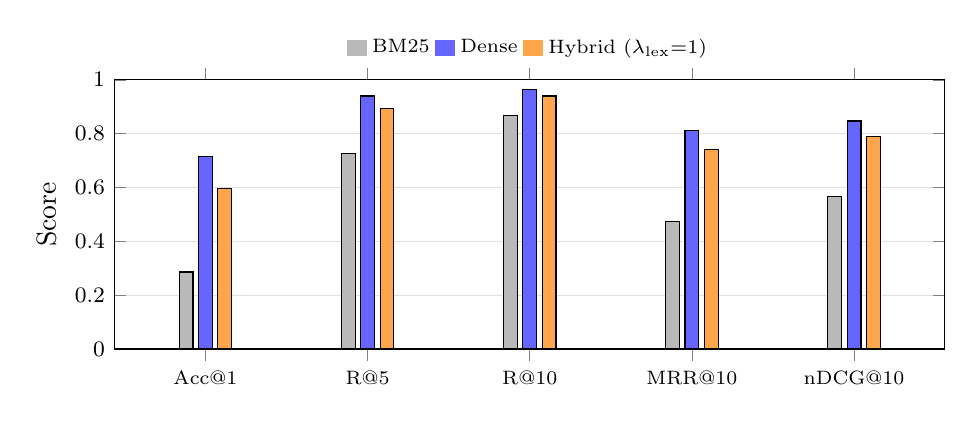
\begin{tikzpicture}
\begin{axis}[
  ybar, bar width=5pt, width=\columnwidth, height=5.0cm,
  ymin=0, ymax=1, ylabel={Score},
  symbolic x coords={Acc@1,R@5,R@10,MRR@10,nDCG@10},
  xtick=data, xticklabel style={font=\scriptsize},
  yticklabel style={font=\footnotesize},
  legend style={font=\scriptsize, at={(0.5,1.04)}, anchor=south, legend columns=3, draw=none},
  legend image code/.code={\draw[#1, draw=none] (0cm,-0.1cm) rectangle (0.25cm,0.1cm);},
  enlarge x limits=0.14, ymajorgrids, grid style={gray!25},
]
\addplot[fill=gray!55] coordinates {(Acc@1,0.286) (R@5,0.726) (R@10,0.869) (MRR@10,0.474) (nDCG@10,0.565)};
\addplot[fill=blue!60] coordinates {(Acc@1,0.714) (R@5,0.940) (R@10,0.964) (MRR@10,0.813) (nDCG@10,0.847)};
\addplot[fill=orange!70] coordinates {(Acc@1,0.595) (R@5,0.893) (R@10,0.940) (MRR@10,0.741) (nDCG@10,0.789)};
\legend{BM25, Dense, Hybrid ($\lambda_{\text{lex}}{=}1$)}
\end{axis}
\end{tikzpicture}
\caption{Accuracy of the three retrieval modes on the Flask benchmark.}
\label{fig:modes}
\end{figure}

Dense retrieval is the strongest mode. It ranks the correct definition first
for 30 of 42 queries (Acc@1 $=0.714$) and within the top five for 40 (R@5
$=0.940$). BM25 ranks only 12 queries correctly at the top. Its failures are
queries whose wording shares little vocabulary with the code: for ``run
before-request hooks, call the view function, then finalize the response'' it
retrieves the test module for request hooks rather than
\texttt{Flask.full\_dispatch\_request}. Fig.~\ref{fig:ranks} shows the full
distribution of the first relevant rank.

\begin{figure}[t]
\centering
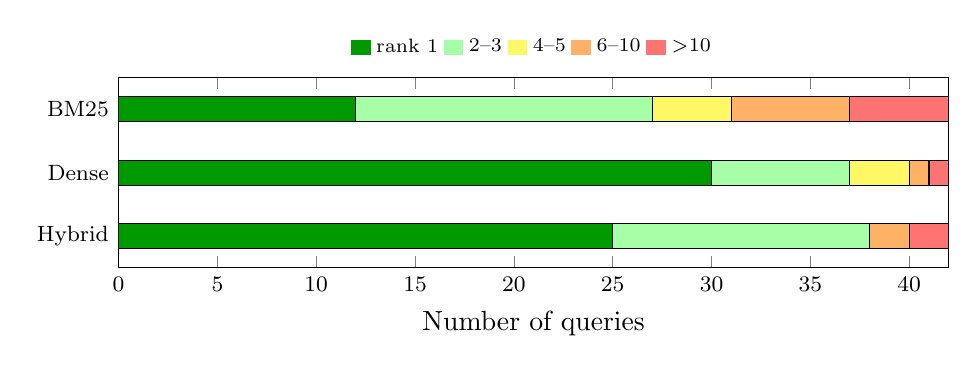
\begin{tikzpicture}
\begin{axis}[
  xbar stacked, bar width=9pt, width=\columnwidth, height=4.0cm,
  xmin=0, xmax=42, xlabel={Number of queries},
  symbolic y coords={Hybrid,Dense,BM25}, ytick=data,
  yticklabel style={font=\footnotesize}, xticklabel style={font=\footnotesize},
  legend style={font=\scriptsize, at={(0.5,1.05)}, anchor=south, legend columns=5, draw=none},
  legend image code/.code={\draw[#1, draw=none] (0cm,-0.1cm) rectangle (0.25cm,0.1cm);},
  enlarge y limits=0.25,
]
\addplot[fill=green!60!black] coordinates {(12,BM25) (30,Dense) (25,Hybrid)};
\addplot[fill=green!35] coordinates {(15,BM25) (7,Dense) (13,Hybrid)};
\addplot[fill=yellow!60] coordinates {(4,BM25) (3,Dense) (0,Hybrid)};
\addplot[fill=orange!60] coordinates {(6,BM25) (1,Dense) (2,Hybrid)};
\addplot[fill=red!55] coordinates {(5,BM25) (1,Dense) (2,Hybrid)};
\legend{rank 1, 2--3, 4--5, 6--10, $>$10}
\end{axis}
\end{tikzpicture}
\caption{Rank of the first relevant result per query ($\lambda_{\text{lex}}=1$ for hybrid).}
\label{fig:ranks}
\end{figure}

\subsection{Effect of the Fusion Weight}
Equal-weight hybrid fusion is \emph{worse} than dense retrieval alone at the top
of the ranking (Acc@1 $0.595$ vs.\ $0.714$; MRR@10 $0.741$ vs.\ $0.813$),
although it slightly improves R@3. Fusion helps 4 queries and hurts 9; the
difference in reciprocal rank is borderline significant ($p = \SigHybP$,
Table~\ref{tab:sig}), whereas the advantage of dense retrieval over BM25 is
highly significant ($p < 0.001$). Fig.~\ref{fig:fusion} shows that accuracy
increases monotonically as the lexical weight decreases. At
$\lambda_{\text{lex}} = 0.05$ hybrid fusion matches dense retrieval (Acc@1
$0.714$) and is marginally higher in MRR@10 ($0.814$ vs.\ $0.813$) and
nDCG@10 ($0.848$ vs.\ $0.847$); at this weight BM25 effectively acts only as a
tie-breaker between near-equal dense scores. This last difference rests on a
single query and is not significant. Under RRF a document's
contribution depends only on its rank, so a weak ranker that places a wrong
chunk first displaces a correct dense result whenever their combined
reciprocal ranks favour it. Table~\ref{tab:sig} reports paired randomisation
tests on per-query reciprocal rank.

\begin{figure}[t]
\centering
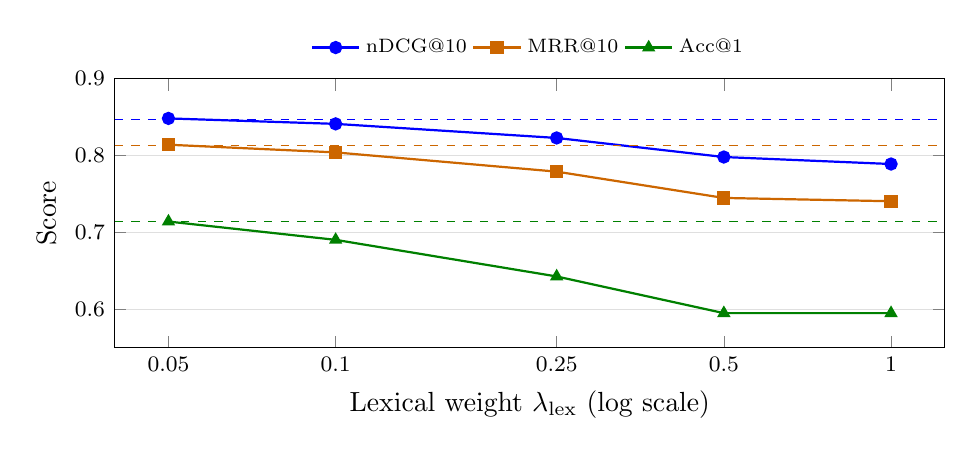
\begin{tikzpicture}
\begin{axis}[
  width=\columnwidth, height=5.0cm,
  xmode=log, log basis x=10, xmin=0.04, xmax=1.25,
  xtick={0.05,0.1,0.25,0.5,1}, xticklabels={0.05,0.1,0.25,0.5,1},
  xlabel={Lexical weight $\lambda_{\text{lex}}$ (log scale)}, ylabel={Score},
  ymin=0.55, ymax=0.9, ymajorgrids, grid style={gray!25},
  xticklabel style={font=\footnotesize}, yticklabel style={font=\footnotesize},
  legend style={font=\scriptsize, at={(0.5,1.04)}, anchor=south, legend columns=3, draw=none},
]
\addplot[mark=*, blue, thick] coordinates {(0.05,0.8484) (0.1,0.8413) (0.25,0.8230) (0.5,0.7982) (1,0.7891)};
\addplot[mark=square*, orange!80!black, thick] coordinates {(0.05,0.8142) (0.1,0.8042) (0.25,0.7792) (0.5,0.7450) (1,0.7407)};
\addplot[mark=triangle*, green!50!black, thick] coordinates {(0.05,0.7143) (0.1,0.6905) (0.25,0.6429) (0.5,0.5952) (1,0.5952)};
\addplot[blue, dashed, domain=0.04:1.25] {0.8474};
\addplot[orange!80!black, dashed, domain=0.04:1.25] {0.8130};
\addplot[green!50!black, dashed, domain=0.04:1.25] {0.7143};
\legend{nDCG@10, MRR@10, Acc@1}
\end{axis}
\end{tikzpicture}
\caption{Hybrid accuracy as a function of the lexical weight. Dashed lines show
dense-only retrieval.}
\label{fig:fusion}
\end{figure}

\begin{table}[t]
\centering
\caption{Paired randomisation tests on per-query reciprocal rank (10\,000 permutations, two-sided)}
\label{tab:sig}
\setlength{\tabcolsep}{3.5pt}
\begin{tabular}{@{}lccc@{}}
\toprule
Comparison & $\Delta$MRR@10 & $p$ & Wins / losses \\
\midrule
\SigRows
\bottomrule
\end{tabular}
\end{table}

\subsection{Ablation Study}
Table~\ref{tab:abl} isolates two design choices. Each ablation is a full
re-index and re-embedding into a separate database with all other settings
fixed (16.8 and 18.9 minutes of indexing, respectively). Because labels
are resolved to definition spans, the same queries and labels apply to every
chunking strategy.

\begin{table}[t]
\centering
\caption{Ablations on the Flask benchmark (dense retrieval unless noted)}
\label{tab:abl}
\setlength{\tabcolsep}{3pt}
\begin{tabular}{@{}lccccc@{}}
\toprule
Configuration & Chunks & Acc@1 & R@5 & MRR@10 & nDCG@10 \\
\midrule
\AblRows
\bottomrule
\end{tabular}
\end{table}

\AblText

\subsection{Replication on Held-Out Queries}
Table~\ref{tab:heldout} (upper part) repeats the three retrieval modes on the
\HoQueries{} held-out queries. The ordering observed on the development set
replicates: dense retrieval (MRR@10 \HoDenseMRR{}) outperforms equal-weight
hybrid fusion (\HoHybMRR{}), which outperforms BM25 (\HoLexMRR{}). On the held-out
set, the dense--hybrid difference is not significant ($p = \HoDenseVsHybP{}$),
so the evidence that equal-weight fusion is harmful remains suggestive rather
than conclusive.

\begin{table*}[t]
\centering
\caption{Development (\NQueries{} queries) and held-out (\HoQueries{} queries) results. ``+ graph'' applies test-aware
graph reranking with the setting selected on the development set ($\beta=\GBeta{}$, $m=\GTop{}$, $\gamma=\GTestW{}$).}
\label{tab:heldout}
\begin{tabular}{@{}lcccccccc@{}}
\toprule
 & \multicolumn{4}{c}{Development} & \multicolumn{4}{c}{Held-out} \\
\cmidrule(lr){2-5}\cmidrule(l){6-9}
Mode & Acc@1 & R@5 & MRR@10 & nDCG@10 & Acc@1 & R@5 & MRR@10 & nDCG@10 \\
\midrule
\HoRows
\bottomrule
\end{tabular}
\end{table*}

\subsection{Test-Aware Graph Reranking}
\textbf{Tuning on the development set.} We swept $\beta \in \{0.5, 1, 2, 4\}$,
$m \in \{5, 10\}$ and $\gamma \in \{1, 0.5\}$ with dense retrieval and selected the
setting with the highest development MRR@10, a rule fixed before the sweep
(ties broken towards the weaker intervention). Fig.~\ref{fig:sweep} shows that
\emph{no} setting improved on dense retrieval for the development set; accuracy
decreases monotonically with $\beta$ and is lower for $m = 10$, because generic
functions called by many tests (URL building, request dispatch) are promoted
into unrelated rankings. The least harmful setting, $\beta = \GBeta{}$,
$m = \GTop{}$, $\gamma = \GTestW{}$, lowers development MRR@10 from \DenseMRR{} to
\DevGDenseMRR{} (\GDevWL{} queries improved/worsened).

\begin{figure}[t]
\centering
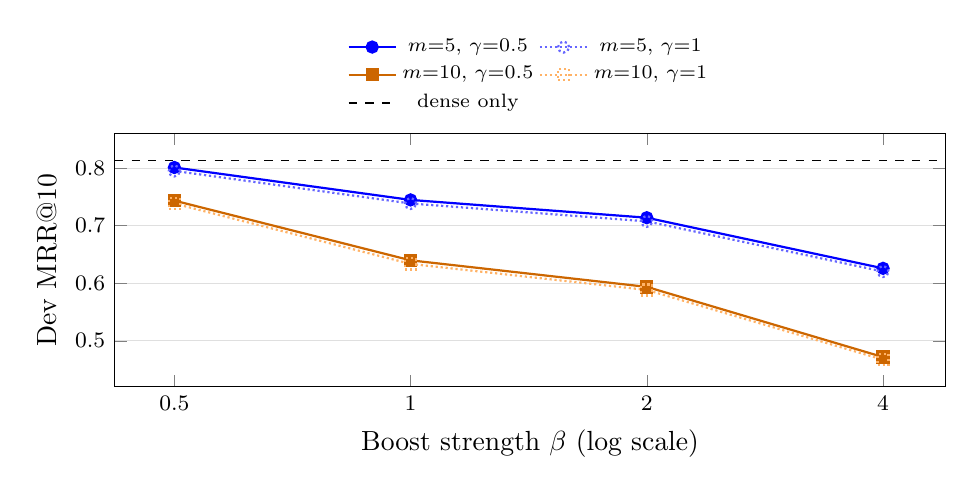
\begin{tikzpicture}
\begin{axis}[
  width=\columnwidth, height=4.8cm,
  xmode=log, log basis x=2, xmin=0.42, xmax=4.8,
  xtick={0.5,1,2,4}, xticklabels={0.5,1,2,4},
  xlabel={Boost strength $\beta$ (log scale)}, ylabel={Dev MRR@10},
  ymin=0.42, ymax=0.86, ymajorgrids, grid style={gray!25},
  xticklabel style={font=\footnotesize}, yticklabel style={font=\footnotesize},
  legend style={font=\scriptsize, at={(0.5,1.04)}, anchor=south, legend columns=2, draw=none},
]
\addplot[mark=*, blue, thick] coordinates {\SweepFiveHalf};
\addplot[mark=o, blue!60, thick, densely dotted] coordinates {\SweepFiveFull};
\addplot[mark=square*, orange!80!black, thick] coordinates {\SweepTenHalf};
\addplot[mark=square, orange!60, thick, densely dotted] coordinates {\SweepTenFull};
\addplot[black, dashed, domain=0.42:4.8] {\SweepBase};
\legend{{$m{=}5$, $\gamma{=}0.5$}, {$m{=}5$, $\gamma{=}1$}, {$m{=}10$, $\gamma{=}0.5$}, {$m{=}10$, $\gamma{=}1$}, {dense only}}
\end{axis}
\end{tikzpicture}
\caption{Development-set sweep of the graph reranker (dense retrieval). The
dashed line is dense retrieval without reranking. Lines for $\gamma=1$ and
$\gamma=0.5$ nearly coincide.}
\label{fig:sweep}
\end{figure}

\textbf{Held-out evaluation.} On the held-out set the same setting
\emph{improves} dense retrieval: Acc@1 rises from \HoDenseAcc{} to
\HoGDenseAcc{} and MRR@10 from \HoDenseMRR{} to \HoGDenseMRR{}, with \GHoWL{}
queries improved/worsened (Table~\ref{tab:heldout}). BM25 also improves, while
hybrid fusion is unchanged because one gain and one loss cancel exactly. The
mechanism is visible in individual queries. For ``maximum size of a cookie
before a warning is issued'', dense retrieval ranks the test
\texttt{test\_max\_cookie\_size} first and the \texttt{Response} class, which
defines \texttt{max\_cookie\_size}, fifth; the reranker follows the test's calls
and moves \texttt{Response} to first place. Similarly,
\texttt{Flask.test\_request\_context} rises from rank 4 to 1.

\textbf{Significance.} None of these differences is statistically significant
(Table~\ref{tab:sig}): $p = \GHoP{}$ on the held-out set, $p = \GDevP{}$ on the
development set and $p = \GPoolP{}$ pooled over all 72 queries (\GPoolWL{}
improved/worsened). The development and held-out estimates also point in
opposite directions. The effect is confined to the minority of queries in which
a test outranks its implementation, so on most queries the reranker changes
nothing. We therefore regard test-aware reranking as a promising but unconfirmed
technique that requires a larger, test-heavy query set to evaluate conclusively.

\subsection{Dependency Graph Correctness}
We audited all import statements of the Python files in the corpus. With naive
path-suffix matching, 343 imports were resolved to repository files, of which
\FalseEdges{} (\FalseEdgePct{}\%) were false positives: standard-library imports
of \texttt{typing} (22), \texttt{logging} (3) and \texttt{json} (3) matched
Flask's own \texttt{flask/typing.py}, \texttt{flask/logging.py} and
\texttt{flask/json/} package. With the package-aware rule of
Section~\ref{sec:deps}, 316 imports are resolved, every resolved edge points to a
module of the repository (\texttt{flask}, relative imports, and the example and
test applications), no import of a repository package is left unresolved, and
no import resolves ambiguously to more than one file. All remaining unresolved
imports name third-party or standard-library modules (e.g.\ \texttt{werkzeug},
\texttt{pytest}, \texttt{os}).

\subsection{Efficiency and Incremental Indexing}
Parsing, chunking, dependency extraction and import resolution of all 194
files take 0.6\,s. Embedding the 1307 chunks on the CPU takes about 18
minutes, an average of 1.22 chunks/s. Cumulative throughput rises from 0.73
chunks/s after 576 chunks to 1.22 chunks/s at the end because the longest
chunks are embedded first. \QueryLatency{} After a configuration change that
forced all 194 files to be re-parsed, the content hash cache matched every
chunk. Re-indexing took 4.7\,s and embedded zero chunks, against about 18
minutes without the cache. Peak memory is bounded
by the encoder, one embedding batch and one scan block, independent of
repository size.

\subsection{Comparison with Existing Work}
Table~\ref{tab:compare} relates our findings to published results.

\begin{table}[t]
\centering
\caption{Comparison with published results}
\label{tab:compare}
\renewcommand{\arraystretch}{1.1}
\begin{tabular}{@{}>{\raggedright\arraybackslash}p{1.9cm}>{\raggedright\arraybackslash}p{2.9cm}>{\raggedright\arraybackslash}p{2.8cm}@{}}
\toprule
Work & Published result & This work \\
\midrule
CoRNStack~\cite{suresh2025cornstack} (CodeRankEmbed) & 77.9 MRR on CodeSearchNet (function-level, docstring queries) & 81.3 MRR@10 on repository-level Flask queries, same model \\
\addlinespace
cAST~\cite{zhang2025cast} & AST chunking: +4.3 Recall@5 over fixed-size chunking (RepoEval) & \CastCompare \\
\addlinespace
RRF~\cite{cormack2009rrf} & Fusion outperforms individual rankers on TREC tasks & Equal-weight fusion \emph{underperforms} the dense ranker ($-0.072$ MRR@10, $p=\SigHybP$) \\
\bottomrule
\end{tabular}
\end{table}

\textbf{CoRNStack.} The CoRNStack authors report 77.9 MRR for CodeRankEmbed on
CodeSearchNet. Using the same model, we obtain 81.3 MRR@10 on our benchmark.
The settings differ: CodeSearchNet ranks isolated functions against
docstring-derived queries with MRR over large candidate pools, whereas we rank
1307 heterogeneous chunks (code, tests and documentation) of a single
repository with a cut-off at 10. The comparable magnitude nevertheless suggests
that the model's zero-shot quality carries over to repository-level search when
chunks align with definitions.

\textbf{cAST.} \CastDiscussion

\textbf{RRF.} Cormack \emph{et al.} found RRF superior to its input rankings.
Our results qualify this: when one ranker is much weaker on the query
distribution (BM25 MRR@10 $0.474$ vs.\ dense $0.813$), equal-weight RRF lowers
top-1 accuracy by 12 percentage points, and the lexical contribution must be
down-weighted by a factor of 20 before fusion is no longer harmful. Fusion
weights should therefore be tuned on held-out queries from the target
distribution rather than fixed at equal values.

% ---------------------------------------------------------------------------
\section{Conclusions and Limitations}

\subsection{Conclusions}
We presented \sys{}, a CPU-only repository-level code retrieval system that
combines syntax-aware chunking, a dependency graph, exact dense search, BM25
and weighted reciprocal rank fusion, with a content-addressed embedding cache
for incremental and reproducible experimentation. On \NQueries{} development
queries over Flask, dense retrieval with CodeRankEmbed reaches \DenseAccOne{}
top-1 accuracy and \DenseRFive{} Recall@5, far ahead of BM25, and the ordering
dense $>$ hybrid $>$ BM25 replicates on \HoQueries{} held-out queries.
Equal-weight hybrid fusion reduces accuracy, and fusion becomes neutral only with
a strongly down-weighted lexical ranker. \AblConclusion{} Test-aware graph
reranking, which follows test-to-code calls to promote implementation code,
improves held-out MRR@10 from \HoDenseMRR{} to \HoGDenseMRR{} without worsening
any held-out query, but slightly lowers development accuracy and is not
statistically significant. A package-aware import rule removes all false-positive
dependency edges of naive path matching. The cache reduces re-indexing after
configuration changes from minutes to seconds.

\subsection{Limitations}
\begin{itemize}
  \item \textbf{Benchmark size and bias.} All 72 queries (42 development,
        30 held-out) were written by the authors, who knew the code base. They paraphrase behaviour and rarely
        contain identifiers, which favours dense over lexical retrieval. Queries
        that quote identifiers or error messages, common in practice, are where
        BM25 is strongest. Differences of a few queries are not statistically
        significant at this sample size (Table~\ref{tab:sig}).
  \item \textbf{Single repository and language.} We evaluate one Python
        project; results may differ for other languages, larger monorepos and
        generated code.
  \item \textbf{Graph reranker evaluation.} The reranker affects only queries
        for which a test ranks highly; with 72 queries, too few such cases exist
        to establish significance. Test detection relies on naming conventions,
        and call resolution is name-based, so generic helpers can be promoted
        spuriously.
  \item \textbf{Single retriever.} Only CodeRankEmbed was evaluated. The
        architecture is model-agnostic, and comparing further checkpoints is
        future work.
  \item \textbf{Throughput.} CPU embedding at about 1.2 chunks/s makes the
        initial indexing of large repositories slow (hours for $10^4$ chunks);
        the exact $O(Nd)$ scan is expected to become a bottleneck beyond about $10^6$ chunks.
  \item \textbf{Heuristic dependency resolution.} Import resolution is
        rule-based and does not model build systems, path aliases, dynamic
        imports or virtual dispatch; call edges are name-based.
\end{itemize}
Future work includes evaluating on issue-derived queries from
SWE-bench~\cite{jimenez2024swebench}, learning query-dependent fusion weights,
evaluating test-aware reranking on a larger, test-heavy query set and with
traceability links that distinguish the functions under test from helpers
called by tests~\cite{white2022tctracer}, and enabling cross-encoder reranking.

% ---------------------------------------------------------------------------
\begin{thebibliography}{00}

\bibitem{husain2019codesearchnet}
Husain, H., Wu, H.H., Gazit, T., Allamanis, M. and Brockschmidt, M., 2019.
CodeSearchNet challenge: Evaluating the state of semantic code search.
\textit{arXiv preprint arXiv:1909.09436}.

\bibitem{gu2018deep}
Gu, X., Zhang, H. and Kim, S., 2018, May. Deep code search. In
\textit{Proceedings of the 40th International Conference on Software
Engineering} (pp. 933--944).

\bibitem{feng2020codebert}
Feng, Z., Guo, D., Tang, D., Duan, N., Feng, X., Gong, M., Shou, L., Qin, B.,
Liu, T., Jiang, D. and Zhou, M., 2020, November. CodeBERT: A pre-trained model
for programming and natural languages. In \textit{Findings of the Association
for Computational Linguistics: EMNLP 2020} (pp. 1536--1547).

\bibitem{guo2022unixcoder}
Guo, D., Lu, S., Duan, N., Wang, Y., Zhou, M. and Yin, J., 2022, May.
UniXcoder: Unified cross-modal pre-training for code representation. In
\textit{Proceedings of the 60th Annual Meeting of the Association for
Computational Linguistics} (pp. 7212--7225).

\bibitem{suresh2025cornstack}
Suresh, T., Reddy, R.G., Xu, Y., Nussbaum, Z., Mulyar, A., Duderstadt, B. and
Ji, H., 2025, April. CoRNStack: High-quality contrastive data for better code
retrieval and reranking. In \textit{Proceedings of the 13th International
Conference on Learning Representations}.

\bibitem{li2025coir}
Li, X., Dong, K., Lee, Y.Q., Xia, W., Zhang, H., Dai, X., Wang, Y. and Tang, R.,
2025, July. CoIR: A comprehensive benchmark for code information retrieval
models. In \textit{Proceedings of the 63rd Annual Meeting of the Association
for Computational Linguistics} (pp. 22074--22091).

\bibitem{karpukhin2020dpr}
Karpukhin, V., Oguz, B., Min, S., Lewis, P., Wu, L., Edunov, S., Chen, D. and
Yih, W.T., 2020, November. Dense passage retrieval for open-domain question
answering. In \textit{Proceedings of the 2020 Conference on Empirical Methods in
Natural Language Processing} (pp. 6769--6781).

\bibitem{robertson2009bm25}
Robertson, S. and Zaragoza, H., 2009. The probabilistic relevance framework:
BM25 and beyond. \textit{Foundations and Trends in Information Retrieval},
3(4), pp.333--389.

\bibitem{cormack2009rrf}
Cormack, G.V., Clarke, C.L. and Buettcher, S., 2009, July. Reciprocal rank
fusion outperforms Condorcet and individual rank learning methods. In
\textit{Proceedings of the 32nd International ACM SIGIR Conference on Research
and Development in Information Retrieval} (pp. 758--759).

\bibitem{nogueira2019passage}
Nogueira, R. and Cho, K., 2019. Passage re-ranking with BERT. \textit{arXiv
preprint arXiv:1901.04085}.

\bibitem{lewis2020rag}
Lewis, P., Perez, E., Piktus, A., Petroni, F., Karpukhin, V., Goyal, N.,
K\"uttler, H., Lewis, M., Yih, W.T., Rockt\"aschel, T., Riedel, S. and
Kiela, D., 2020, December. Retrieval-augmented generation for
knowledge-intensive NLP tasks. In \textit{Advances in Neural Information
Processing Systems 33} (pp. 9459--9474).

\bibitem{zhang2023repocoder}
Zhang, F., Chen, B., Zhang, Y., Keung, J., Liu, J., Zan, D., Mao, Y., Lou, J.G.
and Chen, W., 2023, December. RepoCoder: Repository-level code completion
through iterative retrieval and generation. In \textit{Proceedings of the 2023
Conference on Empirical Methods in Natural Language Processing}
(pp. 2471--2484).

\bibitem{jimenez2024swebench}
Jimenez, C.E., Yang, J., Wettig, A., Yao, S., Pei, K., Press, O. and
Narasimhan, K., 2024, May. SWE-bench: Can language models resolve real-world
GitHub issues? In \textit{Proceedings of the 12th International Conference on
Learning Representations}.

\bibitem{zhang2025cast}
Zhang, Y., Zhao, X., Wang, Z.Z., Yang, C., Wei, J. and Wu, T., 2025, November.
cAST: Enhancing code retrieval-augmented generation with structural chunking
via abstract syntax tree. In \textit{Findings of the Association for
Computational Linguistics: EMNLP 2025} (pp. 8106--8116).

\bibitem{phan2024repohyper}
Phan, H.N., Phan, H.N., Nguyen, T.N. and Bui, N.D.Q., 2024. RepoHyper:
Search-expand-refine on semantic graphs for repository-level code completion.
\textit{arXiv preprint arXiv:2403.06095}.

\bibitem{liu2024graphcoder}
Liu, W., Yu, A., Zan, D., Shen, B., Zhang, W., Zhao, H., Jin, Z. and Wang, Q.,
2024, October. GraphCoder: Enhancing repository-level code completion via
coarse-to-fine retrieval based on code context graph. In \textit{Proceedings of
the 39th IEEE/ACM International Conference on Automated Software Engineering}
(pp. 570--581).

\bibitem{white2022tctracer}
White, R. and Krinke, J., 2022. TCTracer: Establishing test-to-code
traceability links using dynamic and static techniques. \textit{Empirical
Software Engineering}, 27, Article 67.

\end{thebibliography}

\end{document}
